\documentclass[12pt,twoside]{report}

\setcounter{errorcontextlines}{4}

\setlength{\textheight}{240mm}
\addtolength{\topmargin}{-25mm}
\addtolength{\textwidth}{5mm}
\addtolength{\oddsidemargin}{5mm}
\addtolength{\evensidemargin}{-10mm}

%% %%%%%%%%% PACKAGES
%\usepackage{../../skript/gbi}
\usepackage{amsmath}
\usepackage{amssymb}
\usepackage{booktabs}
\usepackage{enumerate}
\usepackage{fancyhdr}
\usepackage{german}
\usepackage{graphicx}
\usepackage[latin1]{inputenc}
\usepackage{pst-all}
\usepackage{latexsym}
\usepackage{mdwlist}
%\usepackage{thwmathligs}
\usepackage{thwpalatino}
\usepackage{euler}
\usepackage{tabularx}
\usepackage{tikz}
\usetikzlibrary{matrix}
%% \usepackage{thwalg}
%\usepackage{thwmathabbrevs}
%\usepackage{thwtextabbrevs}
% \usepackage{url}
\usepackage{array}

\pagestyle{fancy}
\fancyhead{}
\fancyfoot{}
\fancyhead[RO]{{Matr.-Nr.:}\hspace*{40mm}}
\fancyhead[LO]{{Name:}}
\fancyfoot[CE,CO]{\thepage}

\newcommand{\N}{\ensuremath{\mathbb{N}}}
\newcommand{\io}{\ensuremath{\!\mid\!}}

\usepackage[digits]{at}
\usepackage{cmtt}
\newatcommand N[1]{\ensuremath{\langle}\hbox{\textit{#1}}\ensuremath{\rangle}}
\newatcommand T[1]{\hbox{\upshape\mttfamily\bfseries{#1}}}
\newatcommand M[1]{\ensuremath{\big#1}}
\newatcommand .{\ensuremath{\mathop{\hbox{\textbullet}}\,}}
\let\Hash=\#
\renewcommand{\#}[1]{\textup{\texttt{#1}}}
\newcommand{\act}{\ensuremath{\mathit{act}}}
\newcommand{\goto}{\ensuremath{\mathit{goto}}}
\def\strich{\underline{\hspace*{1cm}}}
\def\Strich{\underline{\hspace*{2cm}}}
\def\implies{\Rightarrow}
\def\BoX{\scalebox{3.0}{\Box}}
\def\A{\mathcal{A}}
\def\B{\mathcal{B}}

\def\JANEIN{\qquad ja: \strich\qquad nein: \strich }

\newcounter{afgnr}
\setcounter{afgnr}{1}

\parskip=12pt
\parindent=0pt

\newenvironment{aufgabe}[1][\relax]%
  {\clearpage
    \noindent\textbf{Aufgabe \arabic{afgnr}}%
    \if#1\relax\else{ (#1 Punkte)}\fi
    \\
  }%
  {\addtocounter{afgnr}{1}}%

\begin{document}

\thispagestyle{empty}

\begin{center}
  \bfseries \Large
  Klausur zur Vorlesung \\
  Grundbegriffe der Informatik \\
  1. September 2011 \\[8mm]
  \begin{tabular}{l@{\quad}|c|c|c|}
    \cline{2-4}
    Klausur- &
    \hbox to 20mm{\hss \vrule width 0pt height 8mm depth 1mm}&
    \hbox to 20mm{\hss \vrule width 0pt height 8mm depth 1mm}&
    \hbox to 20mm{\hss \vrule width 0pt height 8mm depth 1mm}\\
    nummer &
    \hbox to 20mm{\hss \vrule width 0pt height 6mm depth 5mm}&
    \hbox to 20mm{\hss \vrule width 0pt height 6mm depth 5mm}&
    \hbox to 20mm{\hss \vrule width 0pt height 6mm depth 5mm}\\
    \cline{2-4}
  \end{tabular}

\end{center}

%\vspace*{5mm}
\def\Q{\hspace*{12mm}}
\begin{center}
  \begin{tabular}[t]{|l|*{8}{c|}}
    \cline{1-5}
    \multicolumn{5}{|l|}{} \\
    \multicolumn{5}{|l|}{Name:} \\
    \multicolumn{5}{|l|}{} \\
    \cline{1-5}
    \multicolumn{5}{|l|}{} \\
    \multicolumn{5}{|l|}{Vorname:} \\
    \multicolumn{5}{|l|}{} \\
    \cline{1-5}
    \multicolumn{5}{|l|}{} \\
    \multicolumn{5}{|l|}{Matr.-Nr.:} \\
    \multicolumn{5}{|l|}{} \\
%     \cline{1-5}
%     \multicolumn{2}{|l|}{} & & & \\
%     \multicolumn{2}{|l|}{Klausur.-Nr.:} & & &\\
%     \multicolumn{2}{|l|}{} & & & \\
    \cline{1-5}
    \multicolumn{8}{c}{ } \\
%    \multicolumn{8}{c}{ } \\
%    \multicolumn{8}{c}{ } \\
%    \multicolumn{8}{c}{ } \\
    \cline{1-8}
    \            &   &   &   &   &   &   &      \\
    Aufgabe      & 1 & 2 & 3 & 4 & 5 & 6 & 7   \\
    \            & \Q& \Q& \Q& \Q& \Q& \Q& \Q  \\
    \cline{1-8}
    \            &   &   &   &   &   &   &      \\
    max. Punkte  & 5 & 5 & 6 & 7 & 5 & 6 & 8    \\
    \            &   &   &   &   &   &   &      \\
    \cline{1-8}
    \            &   &   &   &   &   &   &      \\
    tats. Punkte &   &   &   &   &   &   &      \\
    \            &   &   &   &   &   &   &      \\
  \cline{1-8}
%    \multicolumn{7}{c}{ } \\
%    \multicolumn{7}{c}{ } \\
%    \multicolumn{7}{c}{ } \\
    \multicolumn{8}{c}{ } \\
    \cline{1-4}\cline{6-7}
    \multicolumn{4}{|l|}{ } &
    \multicolumn{1}{c}{ } &
    \multicolumn{2}{|l|}{ } & \multicolumn{1}{c}{ }\\
    \multicolumn{4}{|l|}{Gesamtpunktzahl:} &
    \multicolumn{1}{c}{ } &
    \multicolumn{2}{|l|}{Note:} & \multicolumn{1}{c}{ }\\
    \multicolumn{4}{|l|}{ } &
    \multicolumn{1}{c}{ } &
    \multicolumn{2}{|l|}{ } & \multicolumn{1}{c}{ } \\
    \cline{1-4}\cline{6-7}
  \end{tabular}
\end{center}

%=======================================================================
\def\foobar{\relax}
\def\repeattm{0}

\begin{aufgabe}[5]

  \vspace*{-2\baselineskip}

  \begin {enumerate}
  \item Gegeben sei die formale Sprache $L_1=\bigl(\{\#a,\#b \}^* \cdot
    \{\#c\}\bigr)^*$. Geben Sie alle W�rter der L�nge $2$ in $L_1$ an.

  \item Geben Sie eine Menge $L_2$ von W�rtern an, so dass gilt:
    \[
    L_2\cdot L_2=\{ \#{aa}, \#{aba}, \#{aab}, \#{abab} \}
    \]

  \item Gegeben sei die kontextfreie Grammatik
    $G_3=(\{S,X,Y,Z\},\{\#a,\#b,\#d,\#e,\#f\},S,P)$ mit folgender
    Produktionenmenge
    \begin{align*}
      P = \{\;\;\; & S \to \#aS \mid S\#b \mid \varepsilon \mid X, \\
      &X \to \#d Z \mid Y\#e \mid \#f Y, \\
      & Y \to \varepsilon, \\
      &Z \to \#dX \\
      \}\;\;\;& \\
    \end{align*}
    Geben Sie einen regul�ren Ausdruck an, der genau $L(G_3)$ beschreibt.
  \item Es seien $R, S, T\subseteq M\times M$ bin�re Relationen auf
    einer Menge $M$. Beweisen oder widerlegen Sie (durch Angabe eines
    Gegenbeispiels):
    \[
    R\circ S \cap R\circ T \subseteq R\circ(S\cap T)
    \]
  \end{enumerate}
 
\clearpage
\textit{Weiterer Platz f�r Antworten zu Aufgabe \theafgnr:}
\end{aufgabe}

%=======================================================================
\begin{aufgabe}[5]\\[-0.5\baselineskip]
  In dieser Aufgabe geht es um ungerichtete Graphen ohne Schlingen.

  \begin {enumerate}
  \item Zeichnen Sie alle paarweise nichtisomorphen ungerichteten
    schlingenfreien Graphen mit genau $5$ Knoten und genau $5$ Kanten,
    die einen Weg besitzen, in dem alle Knoten vorkommen.

    Suchen Sie sich einen Ihrer Graphen aus und geben Sie f�r ihn die
    Wegematrix an.
  \item Zeichnen Sie alle paarweise nichtisomorphen ungerichteten
    schlingenfreien Graphen mit genau $6$ Knoten, die alle Grad $1$
    haben.
  \item Wieviele ungerichtete schlingenfreie Graphen mit Knotenmenge
    $V=\{0,1,2,3,4,5\}$ gibt es, bei denen alle Knoten Grad $1$ haben?
  \end{enumerate}

  \vspace*{\baselineskip}

  \textbf{Achtung:} Bei den ersten beiden Teilaufgaben gibt es bei
  Angabe mehrerer isomorpher Graphen Punktabzug. (Aber man kann auf
  keine Teilaufgabe weniger als $0$ Punkte bekommen.)

  \clearpage
  
  \textit{Weiterer Platz f�r Antworten zu Aufgabe \theafgnr:}
\end{aufgabe}

%=======================================================================
\begin{aufgabe}[6]\\[-0.5\baselineskip]  
  Eine Funktion $T(n):\N_0 \to \N_0$ sei rekursiv wie folgt definiert:
  \begin {itemize}
  \item $T(0)=2$
  \item $T(1)=3$
  \item F�r alle $n\in\N_0\smallsetminus\{0,1\}$ sei: \\
    \[ T(n) = 3\cdot T(n-1) -2\cdot T(n-2) \]
  \end{itemize}

  \begin{enumerate}
  \item Geben Sie die Funktionswerte $T(n)$ f�r $n\in\{2,3,4,5,6\}$
    an.
  \item Geben Sie eine geschlossene Formel $F(n)$ (d.\,h.~einen
    arithmetischen Ausdruck) f�r $T(n)$ an.
  \item Beweisen Sie durch Induktion, dass f�r alle $n\in\N_0$ gilt:
    $F(n)=T(n)$.
  \end{enumerate}

\clearpage
\textit{Weiterer Platz f�r Antworten zu Aufgabe \theafgnr:}
\end{aufgabe}

%=======================================================================
\begin{aufgabe}[7]\\[-0.5\baselineskip]  
  In dieser Aufgabe geht es um Huffman-Codierungen.

  \begin {enumerate}
  \item Gegeben sei das Alphabet $A=\{\#a, \#b, \#c, \#d, \#e, \#f,
    \#g\}$ und ein Wort $w\in A^*$ in dem die Symbole mit folgenden
    H�ufigkeiten vorkommen:

    \begin{center}
      \begin{tabular}{*{7}{c}}
        \toprule
        \#a & \#b & \#c & \#d & \#e & \#f & \#g \\
        \midrule
        $11$ & $3$ & $11$ & $24$ & $8$ & $7$ & $36$ \\
        \bottomrule
      \end{tabular}
    \end{center}
    
    \begin{enumerate}
    \item Zeichnen Sie den Huffman-Baum.
    \item Geben Sie die Huffman-Codierung des Wortes $\#{bad}$ an.
    \end{enumerate}
  \item F�r $k\geq 1$ sei ein Alphabet $A=\{ a_0, a_1, \dots, a_k\}$
    mit $k+1$ Symbolen gegeben und ein Text, in dem jedes Symbol $a_i$
    mit H�ufigkeit $2^i$ vorkommt f�r $0\leq i \leq k$.

    Geben Sie die Huffman-Codierungen aller Symbole $a_i$ an.
  \end {enumerate}
    

\clearpage
\textit{Weiterer Platz f�r Antworten zu Aufgabe \theafgnr:}
\end{aufgabe}

%=======================================================================
\begin{aufgabe}[5]\\[-0.5\baselineskip]  
  %
  Es sei $A$ ein nichtleeres Alphabet.

  F�r $x\in A$ und $w\in A^*$ sei $N_x(w)$ die Anzahl der Vorkommen
  des Zeichens $x$ im Wort $w$.

  Wir definieren auf $A^*$ eine bin�re Relation $\sqsubseteq$ 
  wie folgt:
  %
  \[ w_1 \sqsubseteq w_2 \text{\quad genau dann, wenn \quad} \forall
  x\in A: N_x(w_1)\leq N_x(w_2)
  \]

  \begin {enumerate}
  \item Besitzt die Relation $\sqsubseteq$ ein kleinstes Element? \\
    Wenn ja: Geben Sie das kleinste Element an. \\
    Wenn nein: Beweisen Sie, dass es keines gibt.
  \item Besitzt die Relation $\sqsubseteq$ ein gr��tes Element? \\
    Wenn ja: Geben Sie das gr��te Element an. \\
    Wenn nein: Beweisen Sie, dass es keines gibt.
  \item Zeigen Sie, dass die Relation $\sqsubseteq$ nicht
    antisymmetrisch ist, wenn $A$ mindestens zwei Symbole enth�lt.
  \end{enumerate}

\clearpage
\textit{Weiterer Platz f�r Antworten zu Aufgabe \theafgnr:}
\end{aufgabe}
 
%=======================================================================
\begin{aufgabe}[6]\\[-0.5\baselineskip]  
  %
  Die Sprache $L \subseteq \{\#0,\#1\}^*$ sei definiert als die Menge
  aller W\"orter $w$, die die Bin�rzahldarstellung einer durch $3$
  teilbaren Zahl sind.
  \begin {enumerate}
  \item Geben Sie alle W\"orter aus $L$ an, deren L�nge h�chstens $3$
    ist.
  \item Geben Sie einen endlichen Akzeptor an, der $L$ erkennt.

  \item Es sei $L'$ die Menge aller W�rter aus $L$ (!), die L�nge $1$
    haben oder mit dem Symbol \#1 beginnen.

    Geben Sie einen endlichen Akzeptor an, der $L'$ erkennt.
  \end {enumerate}

  Hinweis: Es muss sich um vollst�ndige deterministische endliche
  Akzeptoren handeln wie sie in der Vorlesung definiert wurden.
  
\clearpage
\textit{Weiterer Platz f�r Antworten zu Aufgabe \theafgnr:}
\end{aufgabe}

%=======================================================================
\begin{aufgabe}[8]
  Gegeben sei die folgende Turingmaschine $T$:\\[-1.5\baselineskip] 
  \begin{itemize*}
  \item Zustandsmenge ist $Z=\{s, a_1, a_2, a_3, b_1, b_2, b_3, r\}$.
  \item Anfangszustand ist $s$.
  \item Bandalphabet ist $X=\{\Box,\#a,\#b \}$.
  \item Die Arbeitsweise ist durch folgendes Diagramm festgelegt:\\[\baselineskip]
  \end{itemize*}
  
  \vspace*{-3\baselineskip}

  \noindent
  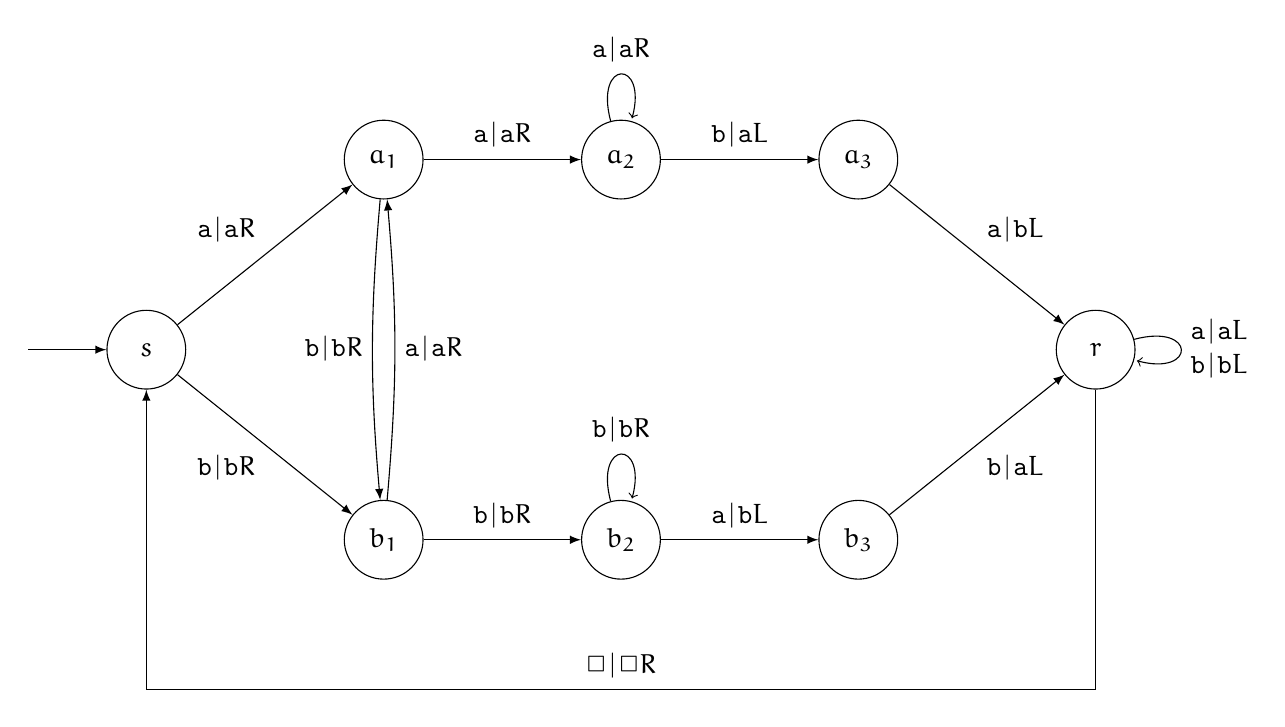
\begin{tikzpicture}[bend angle=5]
      \matrix[matrix of math nodes,column sep=20mm,row sep=14mm,minimum width=10mm,nodes={circle,draw,inner sep=1pt}] {
          & |(a1)| a_1 &  |(a2)| a_2 &  |(a3)| a_3 & \\
           |(s)| s & & & & |(r)| r \\
          & |(b1)| b_1 &  |(b2)| b_2 &  |(b3)| b_3 & \\
         \coordinate (L) {}; & & & & \coordinate (R) {}; \\
      };
      \path[-latex] %(start) edge (s)      
      (s)  edge node[anchor=south east] {$\#a\io\#aR$} (a1)
           edge node[below,anchor=north east] {$\#b\io\#bR$} (b1)
      (a1) edge node[above] {$\#a\io\#aR$} (a2)
           edge[bend right] node[left] {$\#b\io\#b R$} (b1)
      (a2) edge[loop above] node  {$\#a\io\#aR$} ()
           edge node[above] {$\#b\io\#a L$} (a3)
      (a3) edge node[above,anchor=south west]  {$\#a\io\#b L$} (r)
      (b1) edge node[above] {$\#b\io\#bR$} (b2)
           edge[bend right] node[right] {$\#a\io\#a R$} (a1)
      (b2) edge[loop above] node  {$\#b\io\#bR$} ()
           edge node[above] {$\#a\io\#b L$} (b3)
      (b3) edge node[below,anchor=north west]  {$\#b\io\#a L$} (r)
      (r)  edge[loop right] node {\vbox{\hbox{$\#a\io\#a L$}\hbox{$\#b\io\#b L$}}} ()
      ;
      \draw (r) -- (R) ;
      \path (R) edge node[above] {$\Box\io\Box R$} (L) ;
      \draw[-latex] (L) -- (s);
      \draw[latex-] (s) -- +(-1.5,0);
    \end{tikzpicture}

  Die Turingmaschine wird im folgenden benutzt f�r Bandbeschriftungen,
  bei denen zu Beginn der Berechnung auf dem Band ein Wort $w \in
  \{\#a,\#b\}^+$ steht, das von Blanksymbolen umgeben ist.

  Der Kopf der Turingmaschine stehe anfangs auf dem ersten Symbol des
  Eingabewortes.

  
  \begin{enumerate}[1.]
  
  \item Geben Sie f\"ur die Eingabe $\#{aaabbb}$
    folgende Konfigurationen an:
    \begin {itemize}
    \item die Anfangskonfiguration;
    \item die Endkonfiguration;
    \item jede Konfiguration, die in einem Zeitschritt vorliegt,
      nachdem die Turingmaschine vom Zustand $r$ in den Zustand $s$
      gewechselt hat.
    \end {itemize}

    %\foobar
    %\if\repeattm1\turingmachine\\[\baselineskip]\fi

  \item Zu Beginn stehe auf dem Band ein Wort der Form $\#a^k\#b^m$
    mit $k\geq 1$ und $m\geq 0$.  Welches Wort steht am Ende (wenn die
    Turingmaschine gehalten hat) auf dem Band, wenn
    \begin{enumerate}
    \item $k\leq m$ ist?
    \item $k>m$ ist?
    \end{enumerate}
  \item F�r welche Eingabew�rter h�lt die Turingmaschine in Zustand
    $a_1$ an?
  \item Geben Sie eine Funktion $f(n)$ an, so dass die Laufzeit der
    Turingmaschine f�r Eingaben der Form $(\#a\#b)^n$ in
    $\Theta(f(n))$ liegt.
  \item Geben Sie eine Funktion $g(n)$ an, so dass die Laufzeit der
    Turingmaschine f�r Eingaben der Form $\#a^n\#b^n$ in
    $\Theta(g(n))$ liegt.
  \end {enumerate}

\clearpage
\textit{Weiterer Platz f�r Antworten zu Aufgabe \theafgnr:}
\end{aufgabe}
%=======================================================================
%%% Local Variables:
%%% TeX-command-default: "XPDFLaTeX"
%%% TeX-master: szs
%%% End:

%=======================================================================
\end{document}
%%% Local Variables:
%%% TeX-command-default: "XPDFLaTeX"
%%% End:
